\documentclass[tikz,border=6pt]{standalone}
\usepackage{helvet}
\renewcommand{\familydefault}{\sfdefault}
\usetikzlibrary{arrows.meta}
\begin{document}
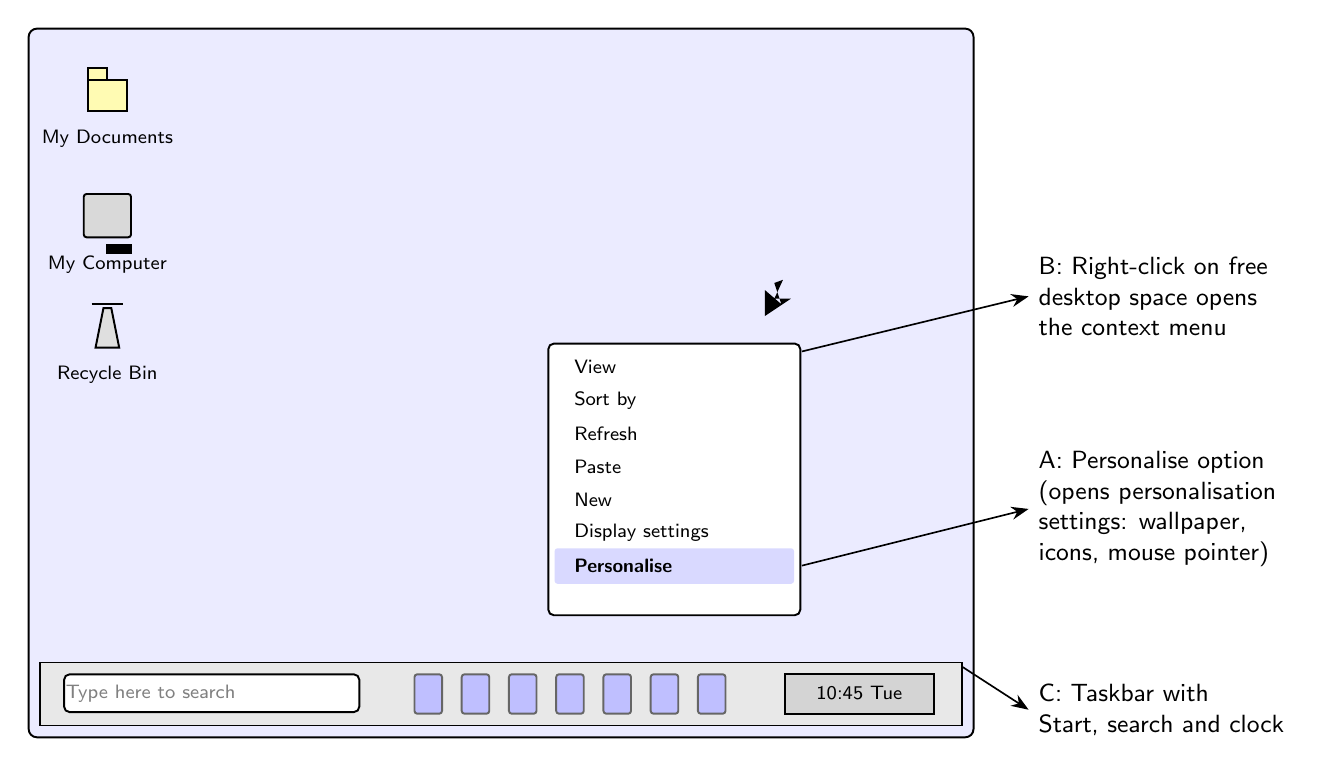
\begin{tikzpicture}[line width=0.7pt, font=\sffamily\small]

% ---- desktop screen (wallpaper) ---------------------------------------------
\draw[fill=blue!8, draw=black, rounded corners=3pt] (0,0) rectangle (12,9.0);

% ---- taskbar (inside the screen, bottom) ------------------------------------
\draw[fill=gray!18, draw=black] (0.15,0.15) rectangle (11.85,0.95);
\draw[fill=white, rounded corners=2pt] (0.45,0.32) rectangle (4.2,0.8); % search box
\node[font=\sffamily\scriptsize, gray] at (1.55,0.56) {Type here to search};
\foreach \x in {4.9,5.5,6.1,6.7,7.3,7.9,8.5} {
  \draw[fill=blue!25, draw=black!60, rounded corners=1pt] (\x,0.3) rectangle (\x+0.35,0.8);
}
\draw[fill=gray!34, draw=black] (9.6,0.3) rectangle (11.5,0.8); % clock box
\node[font=\sffamily\scriptsize] at (10.55,0.56) {10:45  Tue};

% ---- desktop icons (left column, on the wallpaper) --------------------------
% My Documents (folder)
\draw[fill=yellow!30, draw=black] (0.75,7.95) rectangle (1.25,8.35);
\draw[fill=yellow!30, draw=black] (0.75,8.35) rectangle (1.0,8.5);
\node[font=\sffamily\scriptsize, align=center] at (1.0,7.6) {My Documents};
% My Computer (small monitor)
\draw[fill=gray!30, draw=black, rounded corners=1pt] (0.7,6.35) rectangle (1.3,6.9);
\draw[fill=black] (1.0,6.15) rectangle (1.3,6.25);
\node[font=\sffamily\scriptsize, align=center] at (1.0,6.0) {My Computer};
% Recycle Bin (bin)
\draw[fill=gray!25, draw=black] (0.85,4.95) -- (1.15,4.95) -- (1.05,5.45) -- (0.95,5.45) -- cycle;
\draw (0.8,5.5) -- (1.2,5.5); % lid
\node[font=\sffamily\scriptsize, align=center] at (1.0,4.6) {Recycle Bin};

% ---- pointer and right-click position --------------------------------------
\fill[black] (9.35,5.35) -- (9.35,5.68) -- (9.56,5.5) -- (9.47,5.77) -- (9.58,5.81) -- (9.47,5.57) -- (9.68,5.57) -- cycle;

% ---- context menu ------------------------------------------------------------
\draw[fill=white, draw=black, rounded corners=2pt] (6.6,1.55) rectangle (9.8,5.0);
\foreach \l [count=\i from 0] in {View, Sort by, Refresh, Paste, New, Display settings} {
  \node[font=\sffamily\scriptsize, anchor=west] at (6.8,4.7-0.42*\i) {\l};
}
% highlighted Personalise row (drawn separately, once)
\draw[fill=blue!15, draw=none, rounded corners=1pt] (6.68,1.95) rectangle (9.72,2.4);
\node[font=\sffamily\scriptsize\bfseries, anchor=west] at (6.8,2.18) {Personalise};

% ---- callouts ---------------------------------------------------------------
\draw[-{Stealth[length=2.2mm]}, line width=0.6pt] (9.82,4.9) -- (12.7,5.6)
  node[right, font=\sffamily\small, align=left] {B: Right-click on free\\desktop space opens\\the context menu};
\draw[-{Stealth[length=2.2mm]}, line width=0.6pt] (9.82,2.18) -- (12.7,2.9)
  node[right, font=\sffamily\small, align=left] {A: Personalise option\\(opens personalisation\\settings: wallpaper,\\icons, mouse pointer)};
\draw[-{Stealth[length=2.2mm]}, line width=0.6pt] (11.85,0.9) -- (12.7,0.35)
  node[right, font=\sffamily\small, align=left] {C: Taskbar with\\Start, search and clock};

\end{tikzpicture}
\end{document}
